\documentclass[aspectratio=169]{beamer}
% packages
\usepackage{multicol}
\usepackage[T2A]{fontenc}
\usepackage[utf8]{inputenc}
\usepackage[english,russian]{babel}
\usepackage{booktabs}
\usepackage{biblatex}
\usepackage{graphicx}
\usepackage{href-ul}
\usepackage{cmap}
\usepackage{svg}

\usepackage{lipsum}

% math packages
\usepackage{amsmath,amsfonts,amssymb,amsthm,mathtools}
\usepackage{mathtext}
\usepackage{icomma}
\usepackage{floatflt}

% settings
\setbeamertemplate{navigation symbols}{}
\setbeamertemplate{section in toc}[sections numbered]
\setlength{\columnseprule}{0.2pt}

%%%%%%%%%%%%%%%%%%%%%%%%%%%%%%%%%%
% Metropolis Theme Configuration %
%%%%%%%%%%%%%%%%%%%%%%%%%%%%%%%%%%

\usetheme[
    %%% main theme %%%
    titleformat=regular, 
    %%% inner theme %%%
    sectionpage=progressbar, % + slide
    %sectionpage=none, % disables section page
    %%% outer theme %%%
    numbering=fraction,
    progressbar=frametitle,
    %%% color theme %%%
    block=transparent,
    background=light
]{metropolis}

%%%%%%%%%%%%% Title %%%%%%%%%%%%%%

\setbeamertemplate{title page}{
  \begin{minipage}[b][\paperheight]{\textwidth}
    \centering  % <-- Center here
    \ifx\inserttitlegraphic\@empty\else\usebeamertemplate*{title graphic}\fi
    \vfill%
    \ifx\inserttitle\@empty\else\usebeamertemplate*{title}\fi
    \ifx\insertsubtitle\@empty\else\usebeamertemplate*{subtitle}\fi
    \usebeamertemplate*{title separator}
    \ifx\beamer@shortauthor\@empty\else\usebeamertemplate*{author}\fi
    \ifx\insertinstitute\@empty\else\usebeamertemplate*{institute}\fi
    \vspace*{0.5cm}
    \ifx\insertdate\@empty\else\usebeamertemplate*{date}\fi
    \vfill
    \vspace*{1mm}
  \end{minipage}
}

\setbeamertemplate{title}{
%  \raggedright%  % <-- Comment here
  \linespread{1.0}%
  \inserttitle%
  \par%
  \vspace*{0.5em}
}
\setbeamertemplate{subtitle}{
%  \raggedright%  % <-- Comment here
  \insertsubtitle%
  \par%
  \vspace*{0.5em}
}

%%%%%%%%%%%%% Blocks %%%%%%%%%%%%%

% map defaulf block to oldblock
\let\oldblock\block
\let\endoldblock\endblock

% change block by adding smallskip
\renewenvironment{block}[1]
{\begin{oldblock}{#1}
    \smallskip
}
{ 
\end{oldblock}
}

\setbeamerfont{bibliography entry title}{size=}
\setbeamerfont{bibliography entry author}{size=}
\setbeamerfont{bibliography entry location}{size=}
\setbeamerfont{bibliography entry note}{size=}

%%%%%%%%%%%%% Colors %%%%%%%%%%%%%

\setbeamercolor{normal text}{fg=black, bg=white}
\setbeamercolor{progress bar}{fg=normal text.fg, bg=normal text.fg!50!black!30} 
\setbeamercolor{frametitle}{fg=normal text.fg, bg=normal text.bg}
% latin bold lower
\newcommand{\ba}{\mathbf{a}} 
\newcommand{\bc}{\mathbf{c}} 
\newcommand{\be}{\mathbf{e}} 
\newcommand{\bh}{\mathbf{h}} 
\newcommand{\bp}{\mathbf{p}} 
\newcommand{\bt}{\mathbf{t}} 
\newcommand{\bs}{\mathbf{s}} 
\newcommand{\bu}{\mathbf{u}} 
\newcommand{\bv}{\mathbf{v}} 
\newcommand{\bw}{\mathbf{w}} 
\newcommand{\bx}{\mathbf{x}} 
\newcommand{\by}{\mathbf{y}} 
\newcommand{\bz}{\mathbf{z}} 
\newcommand{\bm}{\mathbf{m}} 

% latin bold upper
\newcommand{\bA}{\mathbf{A}} 
\newcommand{\bB}{\mathbf{B}} 
\newcommand{\bC}{\mathbf{C}} 
\newcommand{\bI}{\mathbf{I}} 
\newcommand{\bJ}{\mathbf{J}} 
\newcommand{\bL}{\mathbf{L}} 
\newcommand{\bM}{\mathbf{M}} 
\newcommand{\bP}{\mathbf{P}}
\newcommand{\bQ}{\mathbf{Q}} 
\newcommand{\bR}{\mathbf{R}} 
\newcommand{\bT}{\mathbf{T}} 
\newcommand{\bU}{\mathbf{U}} 
\newcommand{\bV}{\mathbf{V}} 
\newcommand{\bW}{\mathbf{W}} 
\newcommand{\bX}{\mathbf{X}} 
\newcommand{\bY}{\mathbf{Y}} 
\newcommand{\bZ}{\mathbf{Z}} 

% latin cal upper
\newcommand{\cF}{\mathcal{F}} 
\newcommand{\cG}{\mathcal{G}} 
\newcommand{\cI}{\mathcal{I}} 
\newcommand{\cL}{\mathcal{L}} 
\newcommand{\cM}{\mathcal{M}} 
\newcommand{\cN}{\mathcal{N}} 
\newcommand{\cS}{\mathcal{S}} 
\newcommand{\cT}{\mathcal{T}} 
\newcommand{\cW}{\mathcal{W}} 
\newcommand{\cX}{\mathcal{X}} 
\newcommand{\cZ}{\mathcal{Z}} 

% latin bb upper
\newcommand{\bbE}{\mathbb{E}} 
\newcommand{\bbI}{\mathbb{I}} 
\newcommand{\bbP}{\mathbb{P}} 
\newcommand{\bbR}{\mathbb{R}}
\newcommand{\bbX}{\mathbb{X}} 
\newcommand{\bbY}{\mathbb{Y}}
\newcommand{\bbW}{\mathbb{W}} 

% greek bold lower
\newcommand{\bepsilon}{\boldsymbol{\epsilon}} 
\newcommand{\btheta}{\boldsymbol{\theta}} 
\newcommand{\blambda}{\boldsymbol{\lambda}} 
\newcommand{\bpi}{\boldsymbol{\pi}} 
\newcommand{\bmu}{\boldsymbol{\mu}} 
\newcommand{\bsigma}{\boldsymbol{\sigma}} 
\newcommand{\bphi}{\boldsymbol{\phi}} 

% greek bold upper
\newcommand{\bSigma}{\boldsymbol{\Sigma}} 

\DeclareMathOperator*{\argmin}{arg\,min}
\DeclareMathOperator*{\argmax}{arg\,max}

% transpose
\newcommand{\T}{^{\text{\tiny\sffamily\upshape\mdseries T}}}
\addbibresource{../paper/references.bib}
\graphicspath{{figs}}

\usefonttheme[onlymath]{serif}

%%%
\title{Байесовский подход к выбору оптимального размера выборки}
\subtitle{\textcolor{black!50}{Выпускная квалификационная работа бакалавра}}
\author[Н.\,С.~Киселев]{
    Никита Сергеевич Киселев\\
    Научный руководитель: к.ф.-м.н. А.\,В.~Грабовой
}
\institute[МФТИ (НИУ)]{
\small{
    Кафедра интеллектуальных систем ФПМИ МФТИ\\
    Специализация: Интеллектуальный анализ данных\\
    Направление: 03.03.01 Прикладные математика и физика
}}
\date{2024}
%%%

\begin{document}

\maketitle

\begin{frame}{Байесовский подход к определению достаточного размера выборки}
    Исследуется задача определения достаточного размера выборки.
    \begin{block}{Проблема}
        Определение достаточного размера выборки без постановки статистической гипотезы о распределении параметров модели.
    \end{block}
    \begin{block}{Цель}
        Предложить критерий определения достаточного размера выборки. Построить метод, реализующий этот критерий на практике.
    \end{block}
    \begin{block}{Решение}
        Предлагается использовать в качестве критерия
        \begin{enumerate}
            \item Сходимость функции правдоподобия на бутстрапированных подвыборках;
            \item Близость апостериорных распределений параметров на схожих подвыборках.
        \end{enumerate}
    \end{block}
\end{frame}

\begin{frame}{Постановка задачи определения достаточного размера выборки}
    \begin{columns}[t]
    \begin{column}{0.48\textwidth}
        \vspace{-0.5cm}
        \begin{block}{Выборка}
            \vspace{-0.7cm}
            \[ \mathfrak{D}_m = \left\{ (\bx_i, y_i) \right\}, i \in \mathcal{I} = \{ 1, \ldots, m \} \]
            \vspace{-1cm}
            \begin{itemize}
                \item $\bx \in \mathbb{X} \subseteq \mathbb{R}^n$~--- вектор признакового описания объекта;
                \item $y \in \mathbb{Y}$~--- значение целевой переменной.
            \end{itemize}
        \end{block}
        \begin{block}{Вероятностная модель}
            \vspace{-0.7cm}
            \[ p(y, \bw | \bx) = p(y | \bx, \bw) p(\bw): \mathbb{Y} \times \mathbb{W} \times \mathbb{X} \to \mathbb{R}^+ \]
            \vspace{-1cm}
            \begin{itemize}
                \item $p(y | \bx, \bw)$~--- правдоподобие;
                \item $p(\bw)$~--- априорное распределение.
            \end{itemize}
        \end{block}
    \end{column}
    \hspace{0.5cm}
    \vrule
    \hspace{0.5cm}
    \begin{column}{0.48\textwidth}
        \vspace{-0.5cm}
        \begin{block}{Определение}
            Размер выборки $m^*$ называется \underline{достаточным} согласно критерию $T$, если $T$ выполняется для всех $k \geqslant m^*$.
        \end{block}
        \vspace{0.5cm}
        \begin{block}{Требуется}
            \begin{itemize}
                \item Предложить критерий $T$ определения достаточного размера выборки $m^*$;
                \item Построить метод, реализующий критерий $T$ на практике.
            \end{itemize}
        \end{block}
    \end{column}
\end{columns}
\end{frame}

\begin{frame}{Анализ поведения функции правдоподобия}
    \begin{block}{Функция правдоподобия}
        \vspace{-0.5cm}
        \[ L(\mathfrak{D}_m, \mathbf{w}) = p(\by_m | \bX_m, \bw) = \prod_{i=1}^{m} p(y_i | \mathbf{x}_i, \mathbf{w}), \qquad l(\mathfrak{D}_m, \mathbf{w}) = \sum\limits_{i=1}^{m} \log p(y_i | \mathbf{x}_i, \mathbf{w}) \]
        \vspace{-0.5cm}
    \end{block}
    \begin{block}{Оценка максимума правдоподобия}
        \vspace{-0.2cm}
        \[ \hat{\mathbf{w}}_{k} = \argmax_{\bw \in \mathbb{W}} L(\mathfrak{D}_k, \mathbf{w}) \]
        \vspace{-0.5cm}
    \end{block}
    \begin{block}{Определение (\alert{D}-достаточный размер выборки)}
        \[ \forall k \geqslant m^*: \alert{D}(k) = \mathbb{D}_{\hat{\mathbf{w}}_{k}} L(\mathfrak{D}_m, \hat{\mathbf{w}}_{k}) \leqslant \varepsilon \]
    \end{block}
    \begin{block}{Определение (\alert{M}-достаточный размер выборки)}
        \[ \forall k \geqslant m^*: \alert{M}(k) = \left| \mathbb{E}_{\hat{\mathbf{w}}_{k+1}} L(\mathfrak{D}_m, \hat{\mathbf{w}}_{k+1}) - \mathbb{E}_{\hat{\mathbf{w}}_{k}} L(\mathfrak{D}_m, \hat{\mathbf{w}}_{k}) \right| \leqslant \varepsilon \]
    \end{block}
\end{frame}

\begin{frame}{Корректность определения M-достаточного размера выборки}
    Обозначим параметры распределения $\hat{\bw}_k$ следующим образом:
    \begin{itemize}
        \item Математическое ожидание $\mathbb{E} \hat{\bw}_k = \bm_k$;
        \item Матрица ковариации $\mathbb{D} \hat{\bw}_k = \bSigma_k$. 
    \end{itemize}
    \begin{block}{Теорема 1 (Киселев, 2023)}
        Пусть $\| \bm_{k+1} - \bm_k \|_2 \to 0$ и $\| \bSigma_{k+1} - \bSigma_k \|_{F} \to 0$ при $k \to \infty$. Тогда \underline{в модели линейной регрессии} определение M-достаточного размера выборки является корректным. А именно, для любого $\varepsilon > 0$ найдется такой $m^*$, что для всех $k \geqslant m^*$ выполнено $M(k) \leqslant \varepsilon$.
    \end{block}
\end{frame}

\begin{frame}{Анализ апостериорного распределения параметров модели}
    \begin{block}{Определение\footfullcite{MOTRENKO2014743} (Схожие подвыборки)}
        \vspace{-0.2cm}
        Рассмотрим две подвыборки $\mathfrak{D}^1 \subseteq \mathfrak{D}_m$ и $\mathfrak{D}^2 \subseteq \mathfrak{D}_m$. Пусть $\mathcal{I}_1 \subseteq \mathcal{I} = \{ 1, \ldots, m \}$ и $\mathcal{I}_2 \subseteq \mathcal{I} = \{ 1, \ldots, m \}$~--- соответствующие им подмножества индексов.\\
        Подвыборки $\mathfrak{D}^1$ и $\mathfrak{D}^2$ называются \underline{схожими}, если $\left| \mathcal{I}_1 \triangle \mathcal{I}_2 \right| = 1$.
        \vspace{-0.3cm}
    \end{block}
    \begin{block}{Апостериорные распределения на схожих подвыборках}
        \vspace{-0.7cm}
        \begin{align*}
            \mathfrak{D}_k = (\bX_k, \by_k) &\to p_k(\mathbf{w}) = p(\mathbf{w} | \mathfrak{D}_k) \propto p(\mathfrak{D}_k | \mathbf{w}) p(\mathbf{w}) \\
            \mathfrak{D}_{k+1} = (\bX_{k+1}, \by_{k+1}) &\to p_{k+1}(\mathbf{w}) = p(\mathbf{w} | \mathfrak{D}_{k+1}) \propto p(\mathfrak{D}_{k+1} | \mathbf{w}) p(\mathbf{w})
        \end{align*}
        \vspace{-1cm}
    \end{block}
    \begin{block}{Функция близости s-score\footfullcite{Aduenko2017}}
        \vspace{-0.3cm}
        \[ \mathrm{s\text{-}score}(g_1, g_2) = \dfrac{\int_{\bw} g_1(\bw) g_2(\bw) d\bw}{\max_{\mathbf{b}} \int_{\bw} g_1(\bw - \mathbf{b}) g_2(\bw) d\bw} \]
    \end{block}
\end{frame}

\begin{frame}{Близость апостериорных распределений на схожих подвыборках}
    \begin{figure}
        \includesvg[width=0.9\textwidth]{posterior_ru}
    \end{figure}
    \begin{block}{Определение (\alert{KL}-достаточный размер выборки)}
        \[ \forall k \geqslant m^*: \alert{KL}(k) = D_{KL}(p_k \| p_{k+1}) = \int p_k(\bw) \log{\dfrac{p_k(\bw)}{p_{k+1}(\bw)}} d\bw \leqslant \varepsilon \]
    \end{block} 
    \begin{block}{Определение (\alert{S}-достаточный размер выборки)}
        \[ \forall k \geqslant m^*: \alert{S}(k) = \mathrm{s\text{-}score}(p_k, p_{k+1}) \geqslant 1-\varepsilon \]
    \end{block} 
\end{frame}

\begin{frame}{Корректность определений KL- и S-достаточного размера выборки}
    Предположим, что апостериорное распределение является нормальным, то есть $p_k(\bw) = \mathcal{N}\left( \bw | \bm_k, \bSigma_k \right)$.
    \begin{block}{Теорема 2 (Киселев, 2024)}
            Пусть $\| \bm_{k+1} - \bm_k \|_2 \to 0$ и $\| \bSigma_{k+1} - \bSigma_k \|_{F} \to 0$ при $k \to \infty$. Тогда \underline{в модели с нормальным апостериорным распределением параметров} определение KL-достаточного размера выборки является корректным. А именно, для любого $\varepsilon > 0$ найдется такой $m^*$, что для всех $k \geqslant m^*$ выполнено $KL(k) \leqslant \varepsilon$.
    \end{block}
    \begin{block}{Теорема 3 (Киселев, 2024)}
        Пусть $\| \bm_{k+1} - \bm_k \|_2 \to 0$ при $k \to \infty$. Тогда \underline{в модели с нормальным апостериорным распределением параметров} определение S-достаточного размера выборки является корректным. А именно, для любого $\varepsilon > 0$ найдется такой $m^*$, что для всех $k \geqslant m^*$ выполнено $S(k) \geqslant 1-\varepsilon$.
    \end{block}
\end{frame}

\begin{frame}{Модель линейной регрессии с нормальным априорным распределением}
    \begin{block}{Вероятностная модель линейной регрессии}
        \vspace{-0.3cm}
        \[ p(\by, \bw | \bX) = p(\by | \bX, \bw) p(\bw) = \mathcal{N}\left( \by | \bX \bw, \sigma^2 \mathbf{I} \right) \mathcal{N}\left( \bw | \mathbf{0}, \alpha^{-1} \bI \right) \]
        \vspace{-0.7cm}
    \end{block}
    \begin{block}{Апостериорное распределение}
        \vspace{-0.3cm}
        \[ p(\bw | \bX, \by) = \mathcal{N}\left( \bw | \bm, \bSigma \right), \]
        \[ \bSigma = \left( \alpha \bI + \dfrac{1}{\sigma^2} \bX\T \bX \right)^{-1}, \qquad \bm = \left( \bX\T \bX + \alpha \sigma^2 \bI \right)^{-1} \bX\T \by \]
        \vspace{-0.5cm}
    \end{block}
    \begin{block}{Теорема 4 (Киселев, 2024)}
        Пусть множества значений признаков и целевой переменной ограничены, то есть $\exists M \in \mathbb{R}:$ $\| \bx \|_2 \leqslant M$ и $|y| \leqslant M$. Если  $\lambda_{\min}\left( \bX\T_k \bX_k \right) = \omega(\sqrt{k})$ при $k \to \infty$, то \underline{в модели линейной регрессии с нормальным априорным распределением параметров} $\| \bm_{k+1} - \bm_k \|_2 \to 0$ и  $\| \bSigma_{k+1} - \bSigma_k \|_{F} \to 0$ при $k \to \infty$.
    \end{block}
\end{frame}

\begin{frame}{Близость полных байесовских прогнозов для линейной регрессии}
    \begin{block}{Разделение на обучающую и тестовую выборки}
        \vspace{-0.3cm}
        \[ \mathfrak{D}_m = \mathfrak{D}_{m_1}^{\text{train}} \sqcup \mathfrak{D}_{m_2}^{\text{test}} \]
        \vspace{-0.8cm}
    \end{block}
    \begin{block}{Подвыборка тестовой выборки}
        \vspace{-0.3cm}
        \[ \left( \bX_k, \by_k \right) \subset \mathfrak{D}_{m_1}^{\text{train}} \]
        \vspace{-0.8cm}
    \end{block}
    \begin{block}{Теорема 5 (Киселев, 2024)}
        Пусть множества значений признаков и целевой переменной ограничены, то есть $\exists M \in \mathbb{R}:$ $\| \bx \|_2 \leqslant M$ и $|y| \leqslant M$. Если  $\lambda_{\min}\left( \bX\T_k \bX_k \right) = \omega(\sqrt{k})$ при $k \to \infty$, то \underline{в модели линейной регрессии с нормальным априорным распределением параметров}\\
        \vspace{-0.3cm}
        \[ \left\|\mathbb{E}\left[ \mathbf{y}_{\mathrm{test}}|\mathbf{X_{\mathrm{test}}}, \mathbf{X}_{k+1}, \mathbf{y}_{k+1} \right] - \mathbb{E}\left[ \mathbf{y}_{\mathrm{test}}|\mathbf{X_{\mathrm{test}}}, \mathbf{X}_{k}, \mathbf{y}_{k} \right]\right\|_2 \to 0, \]
        \[ \left\|\mathbb{D}\left[ \mathbf{y}_{\mathrm{test}}|\mathbf{X_{\mathrm{test}}}, \mathbf{X}_{k+1}, \mathbf{y}_{k+1} \right] - \mathbb{D}\left[ \mathbf{y}_{\mathrm{test}}|\mathbf{X_{\mathrm{test}}}, \mathbf{X}_{k}, \mathbf{y}_{k} \right]\right\|_F \to 0, \]
        \[ D_{\mathrm{KL}}\left(p(\mathbf{y}_{\mathrm{test}}|\mathbf{X_{\mathrm{test}}}, \mathbf{X}_k, \mathbf{y}_k) \| p(\mathbf{y}_{\mathrm{test}}|\mathbf{X_{\mathrm{test}}}, \mathbf{X}_{k+1}, \mathbf{y}_{k+1})\right) \to 0.  \]
    \end{block}
\end{frame}

\section{Вычислительный эксперимент}

\begin{frame}{Достаточный размер выборки в зависимости от гиперпараметра $\varepsilon$}
    Используются выборки
    \begin{itemize}
        \item Синтетическая регрессия: 500 объектов, 10 признаков;
        \item Синтетическая классификация: 500 объектов, 10 признаков;
        \item Liver Disorders с задачей регрессии: 345 объектов, 5 признаков. 
    \end{itemize}
    Для каждого значения $\varepsilon$ определяется достаточный размер выборки.
    \begin{figure}
        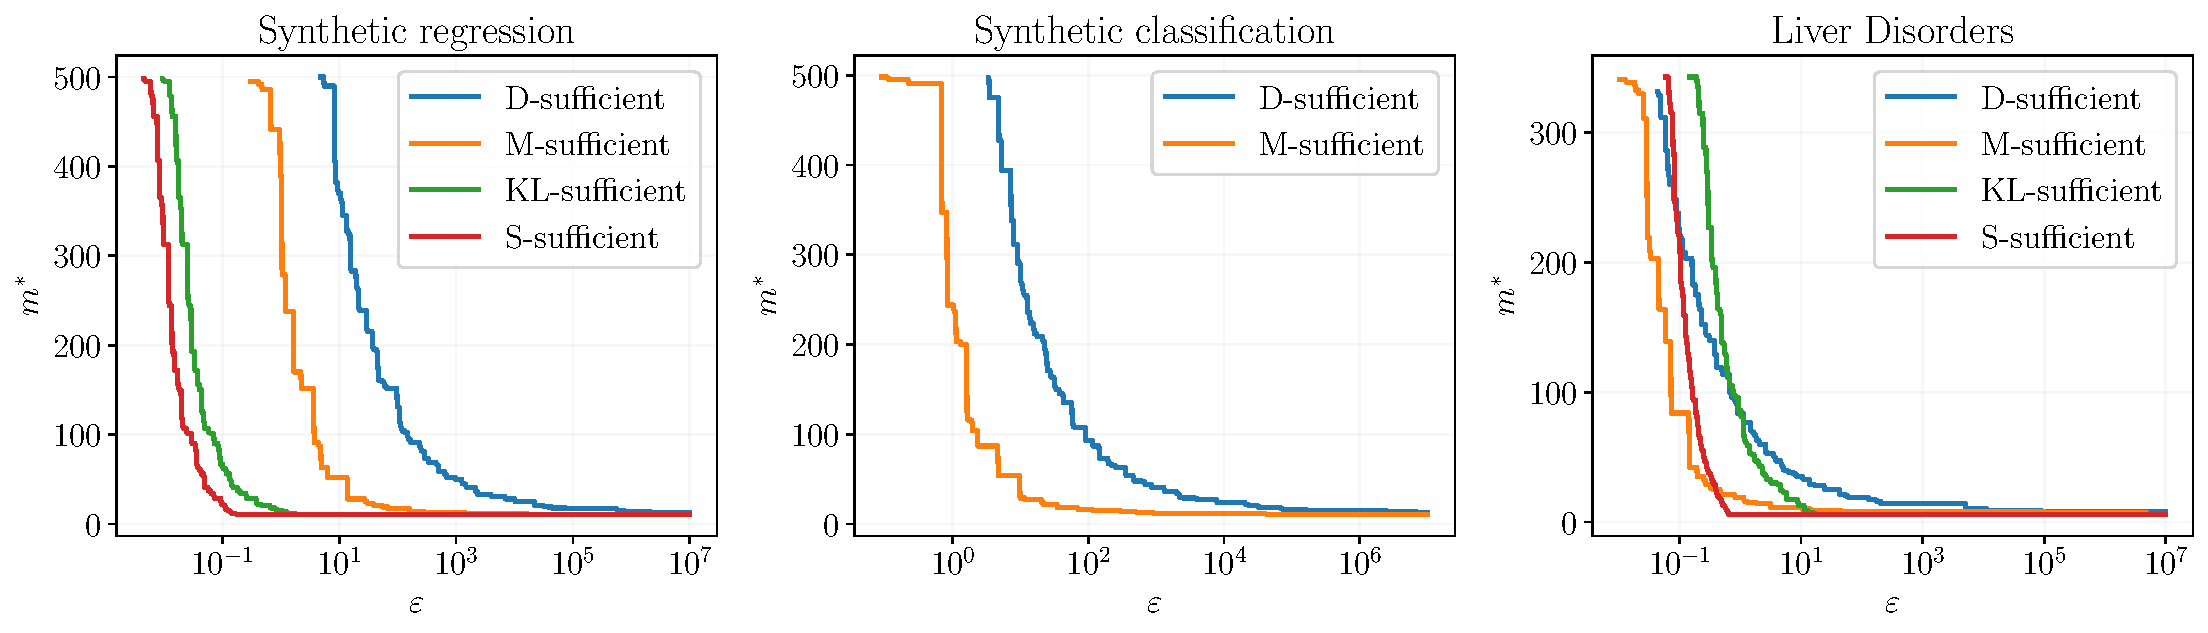
\includegraphics[width=\textwidth]{sufficient-vs-threshold}
    \end{figure}
\end{frame}

\begin{frame}{Сравнение подходов на множестве выборок с задачей регрессии}
    \vspace{-0.3cm}
    Определяется размер выборки, при котором значение метрики уменьшается в 
    \vspace{-0.25cm}
    \begin{itemize}
        \item 1000 раз для D- и M-достаточного размера выборки;
        \item 2 раза для KL- и S-достаточного размера выборки.
    \end{itemize}
    \vspace{-0.1cm}
    Пропуски означают, что первоначальный размер выборки недостаточен.
    \vspace{-0.3cm}
    \scriptsize
    \begin{table}
        \begin{tabular}{ccc|cc|cc}
        \toprule
        Название выборки & Объектов $m$ & Признаков $n$ & D & M & KL & S \\
        \midrule
        Abalone & 4177 & 8 & 96 & 96 & 3921 & 4091 \\
        Auto MPG & 392 & 8 & 15 & 15 & 62 & --- \\
        Automobile & 159 & 25 & 70 & 156 & 156 & --- \\
        Liver Disorders & 345 & 6 & 12 & 19 & --- & --- \\
        Servo & 167 & 4 & 41 & --- & 163 & 163 \\
        Forest fires & 517 & 12 & 208 & --- & 507 & --- \\
        Wine Quality & 6497 & 12 & 144 & 144 & 5305 & 6099 \\
        Energy Efficiency & 768 & 9 & 24 & 442 & --- & --- \\
        Student Performance & 649 & 32 & 129 & 177 & 636 & --- \\
        Facebook Metrics & 495 & 18 & 31 & 388 & 475 & ---  \\
        Real Estate Valuation & 414 & 7 & 15 & 23 & --- & --- \\
        Heart Failure Clinical Records & 299 & 12 & 63 & 224 & 276 & 293 \\
        Bone marrow transplant: children & 142 & 36 & --- & --- & 109 & --- \\
        \bottomrule
        \end{tabular}
    \end{table}
\end{frame}

\begin{frame}{Выносится на защиту}
    \begin{enumerate}
        \item Подходы к определению достаточного размера выборки по
        \begin{itemize}
            \item Сходимости функции правдоподобия на бутстрапированных подвыборках;
            \item Близости апостериорных распределений параметров на схожих подвыборках;
        \end{itemize}
        \item Теоремы о корректности определений
        \begin{itemize}
            \item M-достаточного размера выборки в модели линейной регрессии;
            \item KL-достаточного размера выборки в модели с нормальным апостериорным распределением параметров;
            \item S-достаточного размера выборки в модели с нормальным апостериорным распределением параметров;
        \end{itemize}
        \item Теорема о близости моментов предельного апостериорного распределения в модели линейной регрессии с нормальным априорным распределением параметров;
        \item Теорема о близости полных байесовских прогнозов в модели линейной регрессии с нормальным априорным распределением параметров.
    \end{enumerate}
\end{frame}

\begin{frame}[noframenumbering,plain]{Список работ автора по теме диплома}
    \begin{block}{Публикации ВАК}
        \begin{enumerate}
            \item \textit{\textbf{N. Kiselev}, A. Grabovoy.} Sample Size Determination: Posterior Distributions Proximity // Computational Management Science (на рецензировании).
        \end{enumerate}
    \end{block}
    \begin{block}{Выступления с докладом}
        \begin{enumerate}
            \item Определение достаточного размера выборки по апостериорному распределению параметров модели // 66-я Всероссийская научная конференция МФТИ, 2024.
        \end{enumerate}
    \end{block}
\end{frame}

\end{document}